% ─────────────────────────────────────────────────────────────
% ANEXO — Química de Materiales 1
% Fundamentos y conceptos de apoyo construidos durante el curso.
% Cada sección surge de una duda real resuelta desde el fondo.
% ─────────────────────────────────────────────────────────────

\phantomsection
\label{sec:anexo}
\addcontentsline{toc}{subsection}{Anexo}
\subsection*{\textcolor{blueunam}{Anexo}}

\phantomsection
\label{sec:anexo:tom}
\addcontentsline{toc}{subsubsection}{A.1 Fundamentos de TOM}
\subsubsection*{\textcolor{blueunam}{A.1 Fundamentos de TOM: orbitales, enlazantes,
antienlazantes y deslocalización}}

Este apartado construye desde los principios más básicos por qué existen los orbitales enlazantes y
antienlazantes, por qué uno estabiliza y el otro no, por qué la deslocalización electrónica baja
la energía del sistema, y por qué la polarización sin deslocalización no estabiliza. Todo esto es
la base de la hiperconjugación, el efecto inductivo y la donación por resonancia discutidos en el
texto principal. \\

\phantomsection
\label{sec:anexo:tom:fuerzas}
\textbf{A.1.1 Fuerzas en juego: atracción y repulsión}

Un electrón es una carga negativa. Un núcleo es una carga positiva. Por la ley de Coulomb, cargas
opuestas se atraen: cuanto más cerca está el electrón del núcleo, menor es la energía potencial
del sistema. Los electrones tienden a estar lo más cerca posible del núcleo porque es el estado de
menor energía.

Sin embargo, los electrones también se repelen entre sí (misma carga), y los núcleos se repelen
entre sí. Un enlace existe cuando la suma de las atracciones electrón-núcleo supera la suma de las
repulsiones. Si no las supera, no hay enlace. \\

\phantomsection
\label{sec:anexo:tom:orbital}
\textbf{A.1.2 Qué es un orbital: estado cuántico, no recipiente}

Un orbital no es una región física del espacio que se ``llena'' como un recipiente. Es un
\textit{estado cuántico}: una función de onda $\psi$ que describe la distribución de probabilidad
del electrón. La densidad electrónica en cada punto del espacio es $|\psi|^2$.

\textbf{Principio de exclusión de Pauli:} cada estado cuántico admite máximo dos electrones con
espines opuestos. No importa cuánto ``espacio físico'' haya disponible: el tercer electrón no puede
ocupar el mismo estado aunque sería más estable energéticamente. Debe ir al siguiente estado
disponible. Los electrones ocupan \textit{estados}, no \textit{regiones}. El espacio es continuo;
los estados son discretos. Esta distinción es la esencia de la mecánica cuántica aplicada a la
química. \\

Un átomo no tiene un solo orbital flotando en el espacio: tiene todos sus 
orbitales simultáneamente superpuestos. La mayoría están llenos y no son 
relevantes para la química del átomo en ese contexto. Cuando se representa 
``el orbital del carbono'' en un diagrama de reactividad, se está mostrando 
el que sí participa en la reacción: el orbital frontera. \\

En el caso de los orbitales $p$, no se representa uno solo sino cada 
orientación espacial por separado: $2p_x$, $2p_y$, $2p_z$. Cada nombre 
indica el eje sobre el que se orientan los lóbulos. La forma es idéntica 
en los tres, solo cambia la dirección en el espacio. \\

\begin{figure}[H]
\centering
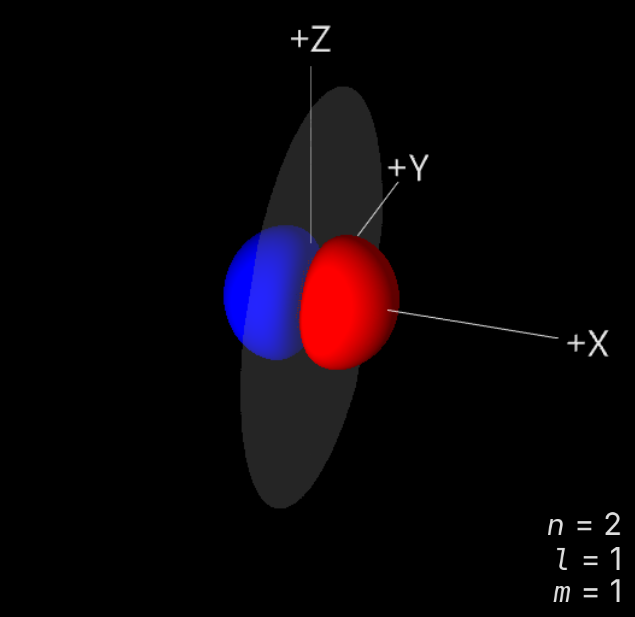
\includegraphics[width=0.35\textwidth]{Imagenes_QM/Orbital_comunmente.png}
\hspace{1cm}
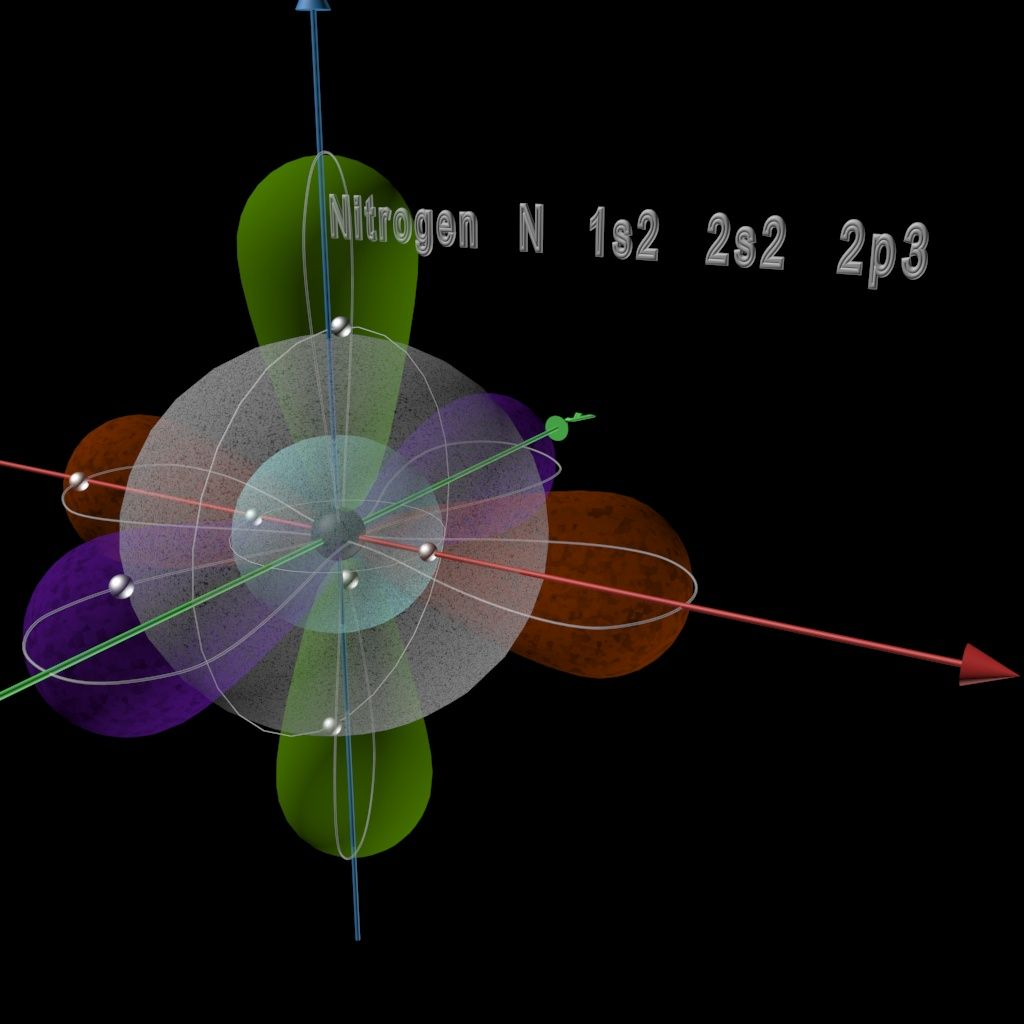
\includegraphics[width=0.45\textwidth]{Imagenes_QM/Orbitales_superpuestos.png}
\caption*{\small Izquierda: representación didáctica estándar de un orbital $2p$ aislado. 
Derecha: el nitrógeno real con todos sus orbitales superpuestos simultáneamente 
($1s^2\,2s^2\,2p^3$). En química se muestra el de la izquierda porque es el 
frontera relevante para la reactividad, no porque sea el único presente.}
\end{figure}

\phantomsection
\label{sec:anexo:tom:cloa}
\textbf{A.1.3 Cómo se forman los orbitales moleculares: CLOA}

Cuando dos átomos se acercan, sus funciones de onda se solapan. La Combinación Lineal de Orbitales
Atómicos (CLOA) establece que $n$ orbitales atómicos producen exactamente $n$ orbitales
moleculares: no se crean ni destruyen, se transforman. Dos orbitales atómicos producen
obligatoriamente un orbital enlazante y uno antienlazante. \\

\phantomsection
\label{sec:anexo:tom:enlazante}
\textbf{A.1.4 Por qué el enlazante es de menor energía}

Las funciones de onda tienen fase (signo matemático). Cuando dos orbitales atómicos se combinan
\textit{en fase} (interferencia constructiva), las funciones de onda se refuerzan en la región
entre los núcleos, aumentando la densidad electrónica ahí.

Un electrón en esa región está simultáneamente cerca de dos núcleos positivos: la atracción
electrostática es la suma de la atracción de ambos, lo cual es muy favorable. Además, esa densidad
actúa como pantalla que reduce la repulsión núcleo-núcleo. El mayor volumen que ocupa el electrón
también baja su energía cinética por el principio de Heisenberg. El sistema baja energía. \\

\phantomsection
\label{sec:anexo:tom:antienlazante}
\textbf{A.1.5 Por qué el antienlazante es de mayor energía}

Cuando dos orbitales se combinan \textit{en desfase} (interferencia destructiva), las funciones de
onda se cancelan entre los núcleos creando un \textbf{nodo}: densidad electrónica cero entre los
núcleos. El electrón está en los lóbulos \textit{externos}, lejos de ambos núcleos en promedio.
Sin pantalla electrónica, los núcleos se repelen sin amortiguación. El sistema sube de energía.

\textbf{Nota importante:} el orbital enlazante y el antienlazante \textit{no} ocupan regiones
separadas del espacio. Ambos se extienden por toda la región alrededor de los núcleos. Lo que
los diferencia es el patrón de densidad: el enlazante tiene su máximo entre los núcleos; el
antienlazante tiene densidad cero en el centro (nodo) y máximos en los extremos.

\begin{center}
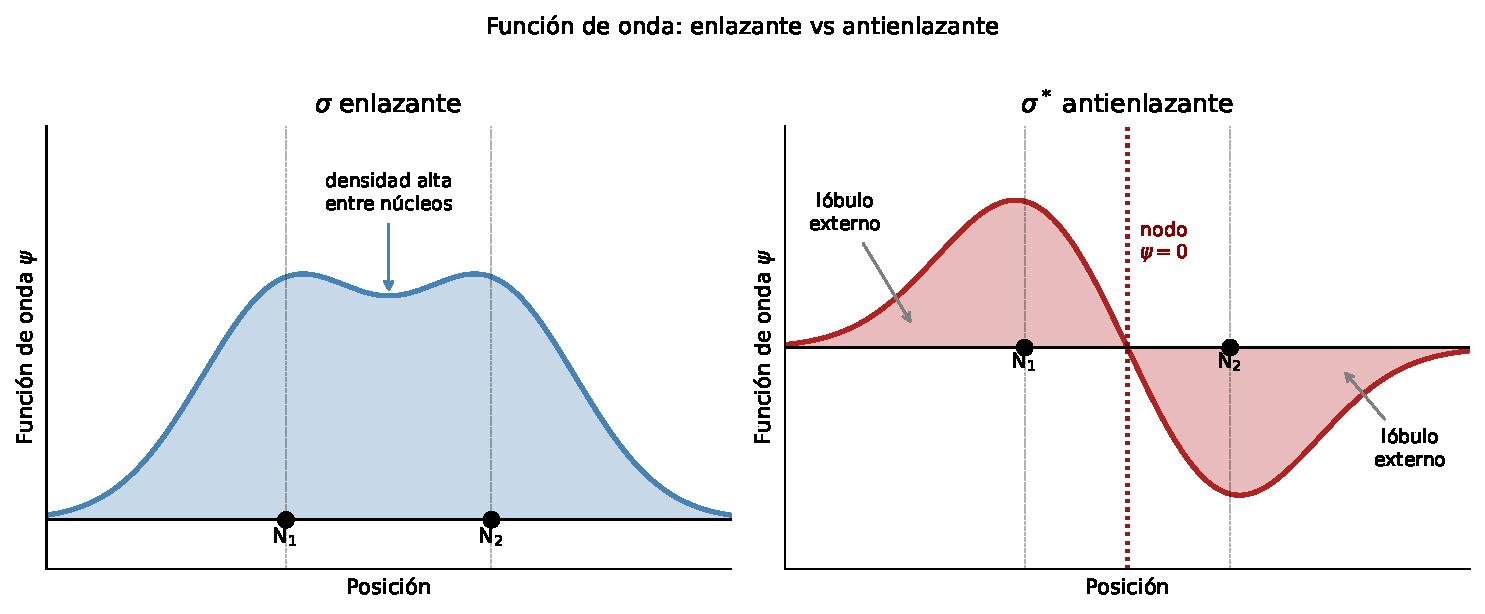
\includegraphics[width=0.85\textwidth]{Imagenes_QM/orbitales_enlace.pdf}
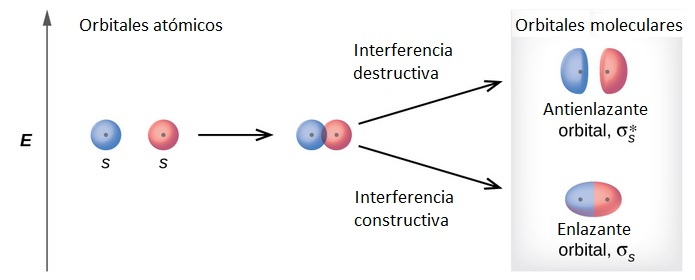
\includegraphics[width=0.85\textwidth]{Imagenes_QM/orbitales.png}
\end{center}

\phantomsection
\label{sec:anexo:tom:pauli}
\textbf{A.1.6 Por qué los electrones no se acumulan en el enlazante}

El enlazante es de menor energía, pero Pauli impide que más de dos electrones lo ocupen. El tercero
debe ir al $\sigma^*$. Esto no es intuitivo clásicamente, pero es consecuencia directa de que los
electrones ocupan estados cuánticos discretos, no espacio continuo. \\

\phantomsection
\label{sec:anexo:tom:orden}
\textbf{A.1.7 Orden de enlace}

\[
\text{O.E.} = \frac{e^- \text{ enlazantes} - e^- \text{ antienlazantes}}{2}
\]

O.E.$=0$: atracciones y repulsiones se cancelan exactamente, la molécula no existe.
Ejemplo: He$_2$ (2 enlazantes $-$ 2 antienlazantes $= 0$). \\

\phantomsection
\label{sec:anexo:tom:heisenberg}
\textbf{A.1.8 Por qué la deslocalización estabiliza: principio de incertidumbre de Heisenberg}

\[
\Delta x \cdot \Delta p \geq \frac{\hbar}{2}
\]

Si el electrón está más confinado en el espacio (menor $\Delta x$), su momento debe ser más
incierto (mayor $\Delta p$), lo que implica mayor energía cinética promedio. Si el electrón puede
ocupar mayor volumen (mayor $\Delta x$), su energía cinética promedio disminuye.

\textbf{Deslocalización:} extiende la nube del electrón hacia mayor volumen $\rightarrow$ menor
energía cinética por Heisenberg $\rightarrow$ sistema más estable.

\textbf{Polarización} (efecto inductivo): contrae la nube hacia un átomo electronegativo sin cambio
de orbital $\rightarrow$ menor volumen efectivo $\rightarrow$ mayor energía cinética $\rightarrow$
desestabiliza en radicales. \\

Mecanismo unificador de los efectos electrónicos según la especie:

\begin{center}
\small
\begin{tabular}{p{3.5cm}p{3cm}p{2cm}p{2cm}}
\hline
\textbf{Efecto} & \textbf{Mecanismo} & \textbf{Rad./Cat.} & \textbf{Carbanión} \\
\hline
Hiperconj. positiva & $\Delta x\uparrow$, $E_k\downarrow$ & Estabiliza & Desestabiliza \\
Hiperconj. negativa & $\Delta x\uparrow$, $E_k\downarrow$ & Estabiliza & Desestabiliza \\
Donación resonancia & $\Delta x\uparrow$, $E_k\downarrow$ & Estabiliza & Desestabiliza \\
Efecto inductivo & Heisenberg$\uparrow$ + Coulomb & Desestabiliza & Estabiliza \\
\hline
\end{tabular}
\normalsize
\end{center}

\textbf{Nota sobre el inductivo en carbaniones:} el efecto inductivo opera simultáneamente por
dos mecanismos opuestos. Por Heisenberg, contrae la nube electrónica aumentando la energía cinética,
lo que desestabiliza. Por Coulomb, retira el exceso de carga negativa del carbono central,
reduciendo la repulsión electrón-electrón, lo que estabiliza. En carbaniones el efecto Coulomb
supera al efecto Heisenberg y el resultado neto es estabilización. En radicales no hay exceso de
carga que aliviar, y Heisenberg domina sin competencia: el inductivo desestabiliza. \\

\phantomsection
\label{sec:anexo:tom:somo}
\textbf{A.1.9 El SOMO semilleno como estado de equilibrio}

El \textsc{somo} con un electrón es un estado intermedio estable. Añadirle un electrón lo acercaría
a un carbanión (exceso de carga negativa, menos estable). Quitarle el único electrón lo convertiría
en un carbocatión (déficit de carga, menos estable). Cualquier desviación del estado semilleno
desestabiliza. Por eso en radicales la deslocalización estabiliza no porque ``done carga'' al
\textsc{somo}, sino porque extiende el volumen del electrón que ya está ahí, bajando su energía
cinética sin alterar la ocupación del estado. \\

\phantomsection
\label{sec:anexo:tom:conexion}
\textbf{A.1.10 Conexión con los efectos del texto principal}

\begin{itemize}
\item \textbf{Hiperconjugación positiva:} los hidrógenos $\beta$ (átomos H unidos al carbono
$\alpha$, es decir a dos enlaces del carbono radical) solapan con el \textsc{somo}. El electrón
desapareado se extiende hacia esos enlaces. Mayor volumen, menor energía cinética, estabiliza.
\item \textbf{Hiperconjugación negativa:} el electrón del \textsc{somo} se extiende hacia el
$\sigma^*$ vacío del enlace C--H vecino alineado. Mayor volumen, menor energía cinética,
estabiliza. Contribuye a geometría ligeramente piramidal.
\item \textbf{Efecto inductivo (F en posición $\alpha$):} el F atrae la nube del \textsc{somo}
hacia sí. El electrón no se transfiere, solo se contrae espacialmente. Menor volumen, mayor
energía cinética, desestabiliza.
\item \textbf{Donación por resonancia (F en posición $\beta$):} el par libre del F solapa con
el \textsc{somo}. El electrón se extiende hacia ese par libre. Mayor volumen, estabiliza. Este
efecto compite con el inductivo del mismo F.
\end{itemize}

\phantomsection
\label{sec:anexo:tom:solapamiento}
\textbf{A.1.11 Por qué el solapamiento extiende la nube}

Cada orbital atómico es una función de onda $\psi$ localizada alrededor de su núcleo. Cuando dos
orbitales se acercan geométricamente y sus fases coinciden, las funciones de onda se suman
constructivamente. El orbital molecular resultante tiene mayor amplitud en esa región extendida,
y como la densidad es $|\psi|^2$, el electrón tiene mayor probabilidad de estar en ese volumen
más amplio.

Este solapamiento no forma un enlace nuevo. Es simplemente que las funciones de onda matemáticas
se superponen en el espacio por estar geométricamente alineadas y en fase. El electrón no se
transfiere, solo tiene mayor probabilidad de existir en mayor volumen. Por eso se llama
deslocalización parcial: la interacción es más débil que un enlace $\pi$ real (que requiere dos
electrones). \\

\textbf{Nota final de A.1:} la hibridación ($sp^2$, $sp^3$) y la \textsc{tev} son modelos
matemáticos sin existencia física propia. \textsc{tom} describe los electrones como estados
cuánticos moleculares sin necesidad de hibridación como concepto separado. El carácter $s$ de
un orbital es un concepto nativo de \textsc{tom} más fundamental que la hibridación discreta.

\phantomsection
\label{sec:anexo:tom:frontera}
\textbf{A.1.12 Orbitales frontera y reactividad}

De todos los orbitales superpuestos de un átomo, la química se simplifica 
enormemente mirando solo el \textbf{orbital frontera}: el que participa 
en la reacción. Según el contexto:
\begin{itemize}
\item \textbf{HOMO} (Highest Occupied Molecular Orbital): orbital lleno 
de mayor energía. Es desde donde dona el nucleófilo.
\item \textbf{LUMO} (Lowest Unoccupied Molecular Orbital): orbital vacío 
de menor energía. Es donde acepta el electrófilo.
\item \textbf{SOMO} (Singly Occupied Molecular Orbital): orbital con un 
solo electrón. Es el orbital del radical.
\end{itemize}

Los demás orbitales están ahí pero no determinan la reactividad en ese 
momento. Por eso en el carbocatión $sp^2$ se muestra el $2p_z$ vacío: 
es el LUMO, donde ataca el nucleófilo. En el radical se muestra el SOMO 
porque ahí está el electrón desapareado.

% ─────────────────────────────────────────────────────────────

\phantomsection
\label{sec:anexo:quiralidad}
\addcontentsline{toc}{subsubsection}{A.2 Quiralidad, enantiómeros y mezclas racémicas}
\subsubsection*{\textcolor{blueunam}{A.2 Quiralidad, enantiómeros y mezclas racémicas}}

Este apartado surge del análisis de la $SN^1$, que genera mezclas racémicas. Para entender
por qué, es necesario comprender qué es la quiralidad y cómo se relaciona con los isómeros
y las mezclas racémicas. \\

\phantomsection
\label{sec:anexo:quiralidad:isomeros}
\textbf{A.2.1 Isómeros}

Los isómeros son moléculas con la misma fórmula molecular pero diferente disposición de átomos.
Existen varios tipos:

\begin{itemize}
\item \textbf{Isómeros constitucionales:} difieren en la conectividad de los átomos.
\item \textbf{Estereoisómeros:} misma conectividad pero diferente disposición espacial.
Incluyen enantiómeros, diastereómeros y conformacionales.
\item \textbf{Enantiómeros:} estereoisómeros que son imágenes especulares no superponibles.
Solo existen cuando la molécula es quiral.
\item \textbf{Diastereómeros:} estereoisómeros que no son imágenes especulares entre sí.
\end{itemize}

\phantomsection
\label{sec:anexo:quiralidad:quiral}
\textbf{A.2.2 Quiralidad}

Un objeto es quiral cuando no es superponible a su imagen especular. En química, una molécula es
quiral cuando tiene al menos un \textbf{carbono quiral}: un carbono unido a cuatro sustituyentes
\textit{diferentes}. La quiralidad es una propiedad de la molécula, no un tipo de isomería.

Una molécula quiral no tiene propiedades físicas o químicas diferentes a su enantiómero en un
entorno aquiral. La diferencia aparece solo cuando interactúa con algo también quiral:

\begin{itemize}
\item \textbf{Luz polarizada:} un enantiómero la rota hacia la derecha (+) y el otro hacia la
izquierda ($-$). Esta propiedad se llama actividad óptica.
\item \textbf{Receptores biológicos:} los receptores son quirales, por eso un enantiómero puede
ser activo farmacológicamente y el otro inactivo o tóxico.
\item \textbf{Reactivos quirales:} reaccionan a velocidades diferentes con cada enantiómero.
\end{itemize}

\phantomsection
\label{sec:anexo:quiralidad:rs}
\textbf{A.2.3 Nomenclatura R y S}

Los enantiómeros se nombran según la configuración absoluta del carbono quiral usando las reglas
de Cahn-Ingold-Prelog (\textsc{cip}):

\begin{enumerate}
\item Asignar prioridades a los cuatro sustituyentes según número atómico (mayor $Z$ = mayor
prioridad).
\item Orientar la molécula con el sustituyente de menor prioridad apuntando hacia atrás.
\item Trazar una flecha de mayor a menor prioridad (1→2→3):
\begin{itemize}
\item Sentido horario → configuración \textbf{R} (\textit{rectus})
\item Sentido antihorario → configuración \textbf{S} (\textit{sinister})
\end{itemize}
\end{enumerate}

\phantomsection
\label{sec:anexo:quiralidad:rac}
\textbf{A.2.4 Mezcla racémica}

Una mezcla racémica es una mezcla en proporción 1:1 de los dos enantiómeros de un compuesto quiral.
No es un tipo de isomería sino una mezcla física. Se denota como $(\pm)$ o \textit{rac-}. No tiene
actividad óptica porque las rotaciones de ambos enantiómeros se cancelan exactamente. \\

\phantomsection
\label{sec:anexo:quiralidad:sn}
\textbf{A.2.5 Por qué $SN^1$ genera mezclas racémicas y $SN^2$ no}

En $SN^1$, el carbocatión intermedio es $sp^2$ y plano. El nucleófilo puede atacar con igual
probabilidad por la cara superior o inferior del orbital $p$ vacío, produciendo ambos enantiómeros
R y S en proporción 1:1: mezcla racémica.

En $SN^2$, el nucleófilo ataca exclusivamente por el lado opuesto al grupo saliente (ataque anti),
produciendo inversión de configuración (\textbf{inversión de Walden}): si el sustrato es R, el
producto es S, y viceversa. Un solo enantiómero.

\begin{center}
\small
\begin{tabular}{lll}
\hline
\textbf{Mecanismo} & \textbf{Estereoquímica} & \textbf{Resultado} \\
\hline
$SN^1$ & Ataque por ambas caras del carbocatión plano & Mezcla racémica $(\pm)$ \\
$SN^2$ & Ataque anti, inversión de Walden & Un solo enantiómero \\
\hline
\end{tabular}
\normalsize
\end{center}

\phantomsection
\label{sec:anexo:nucleofilicidad}
\addcontentsline{toc}{subsubsection}{A.3 Nucleofilicidad y polarizabilidad}
\subsubsection*{\textcolor{blueunam}{A.3 Nucleofilicidad y polarizabilidad}}

\phantomsection
\label{sec:anexo:nucleofilicidad:polar}
\textbf{A.3.1 Polarizabilidad}

La polarizabilidad es qué tan fácil se distorsiona la nube electrónica de 
un átomo bajo la influencia de un campo eléctrico externo. En átomos grandes, 
los electrones de valencia están lejos del núcleo y el efecto apantallante 
de los electrones internos reduce la atracción nuclear sobre ellos, haciendo 
que la nube sea extensa y fácil de deformar. En átomos pequeños la nube es 
compacta y rígida, más difícil de distorsionar.

Factores que aumentan la polarizabilidad:
\begin{itemize}
\item \textbf{Tamaño:} más grande $\Rightarrow$ más polarizable. 
Los electrones externos están más lejos del núcleo y menos atraídos por él.
\item \textbf{Electronegatividad baja:} el átomo retiene menos sus electrones 
y los dona más fácilmente.
\item \textbf{Número de electrones:} más electrones $\Rightarrow$ más 
apantallamiento $\Rightarrow$ electrones externos menos atraídos.
\end{itemize}

\phantomsection
\label{sec:anexo:nucleofilicidad:carga}
\textbf{A.3.2 Nucleofilicidad: carga vs polarizabilidad}

La nucleofilicidad no depende solo de la carga negativa sino también de la 
polarizabilidad. Hay una competencia entre dos efectos:

\begin{itemize}
\item \textbf{A favor de la carga:} mayor densidad de carga negativa 
$\Rightarrow$ mayor atracción electrostática hacia el electrófilo.
\item \textbf{A favor de la polarizabilidad:} nube más distorsionable 
$\Rightarrow$ mejor solapamiento orbital con el $\sigma^*$ del sustrato 
en el estado de transición de $SN^2$.
\end{itemize}

En $SN^2$ domina el \textbf{solapamiento orbital} (factor cinético). 
Por eso \ce{I-} es mejor nucleófilo que \ce{F-} aunque \ce{F} tenga 
mayor carga negativa: el \ce{I-} es grande y polarizable, puede 
distorsionar su nube para solapar bien con el $\sigma^*$ del C--X 
sin repeler tanto a los electrones del enlace. El \ce{F-} es pequeño 
y rígido, su densidad concentrada repele fuertemente antes de llegar 
al $\sigma^*$.

\phantomsection
\label{sec:anexo:nucleofilicidad:cn}
\textbf{A.3.3 El caso del \ce{CN-}: nucleófilo ambidente}

El \ce{CN-} puede atacar por el C o por el N. La carga negativa está 
en el N, lo que sugeriría ataque por N. Sin embargo en $SN^2$ con 
disolvente aprótico ataca por el \textbf{C} porque:

\begin{itemize}
\item El C es más polarizable que el N (menos electronegativo, retiene 
menos sus electrones).
\item Mayor polarizabilidad $\Rightarrow$ mejor solapamiento con el 
$\sigma^*$ del C--X en el estado de transición.
\item La polarizabilidad supera a la ventaja electrostática del N.
\end{itemize}

El producto es un nitrilo R--CN. En condiciones donde domina la 
electrostática (iónicas, termodinámicas) puede atacar por N dando 
isocianuro R--NC.

\phantomsection
\label{sec:anexo:nucleofilicidad:electro}
\textbf{A.3.4 Nucleófilo y electrófilo desde electrostática}

La atracción entre nucleófilo y electrófilo es \textbf{mutua}: ambos 
se atraen simultáneamente por electrostática. La convención de que 
``el nucleófilo ataca al electrófilo'' es solo una elección de 
perspectiva: se sigue el movimiento de los \textbf{electrones}, 
que van de donde sobran hacia donde faltan. Si se siguiera el 
movimiento del ``hueco'' electrónico la dirección sería opuesta, 
pero la física es la misma.

El sitio nucleofílico o electrofílico no tiene que ser toda la 
molécula. Es el átomo o enlace con mayor o menor densidad electrónica 
disponible. Ejemplos: en el etóxido \ce{CH3CH2O-} el nucleófilo es 
el \ce{O-}, no toda la molécula. En el benceno el nucleófilo es el 
sistema $\pi$, no los carbonos individualmente.

\phantomsection
\label{sec:anexo:nucleofilicidad:homo}
\textbf{A.3.5 $SN^2$ desde TOM: interacción HOMO-LUMO}

En $SN^2$ lo que realmente ocurre es una interacción 
\textbf{HOMO-LUMO}: el par libre del nucleófilo (HOMO) solapa con 
el $\sigma^*$ del enlace C--X (LUMO) por el lado opuesto al grupo 
saliente. Al llenarse el $\sigma^*$, el enlace C--X se debilita y 
se rompe simultáneamente con la formación del nuevo enlace C--Nu.

El ataque debe ser \textbf{anti a 180°} porque el lóbulo de mayor 
densidad del $\sigma^*$ está en el lado opuesto al X. Sin esa 
alineación no hay solapamiento y la reacción no ocurre.

La interacción HOMO-LUMO siempre estabiliza el sistema: el orbital 
de menor energía baja más de lo que sube el de mayor energía. Por 
eso la reacción es favorable a pesar de que el $\sigma^*$ tiene más 
energía que el $\sigma$.